% use no footline.
% \begin{frame}[plain, noframenumbering]{Outline}
% 	\tableofcontents
% \end{frame}
%%%%%%%%%%%%%%%%%%%%%%%%%%%%%%%%%%%%%%%%%%%%%%%%%%%%%%
\section{Apache Spark}

\begin{frame}
\frametitle{Chapter Objectives}

\begin{itemize}
	\item Understand the fundamentals of Apache Spark. \pause
	\item Build data processing applications using Apache Spark. \pause
	\item Understand Apache Spark APIs (RDD, DataFrames, and Datasets). \pause
	\item Optimize and tune Apache Spark applications. \pause
	\item Build streaming applications using Apache Spark. \pause
	\item Build scalable machine learning applications using Apache Spark MLlib. \pause
	\item Deploy Apache Spark in production environments. \pause
\end{itemize}

\end{frame}

%%%%%%%%%%%%%%%%%%%%%%%%%%%%%%%%%%%%%%%%%%%%%%%%%%%%%%
\subsection{Course References}
\begin{frame}
	\frametitle{\subsecname}
	\begin{itemize}
		\item \href{https://pages.databricks.com/rs/094-YMS-629/images/LearningSpark2.0.pdf}{Learning Spark, 2nd Edition} By Jules S. Damji, Brooke Wenig, Tathagata Das, Denny Lee. \pause
		\item \href{https://learning.oreilly.com/library/view/spark-the-definitive/9781491912201/}{Spark: The Definitive Guide} By Bill Chambers, Matei Zaharia. \pause
		\item Random blog posts. \pause
	\end{itemize}
	\end{frame}
%%%%%%%%%%%%%%%%%%%%%%%%%%%%%%%%%%%%%%%%%%%%%%%%%%%%%%

\subsection{Course Prerequisites}
\begin{frame}
\frametitle{\subsecname}
Before beginning this course, participants should have:
\begin{itemize}
    \item Experience in programming using Python.  \pause
    \item Basic programming skills using shell.  \pause
    \item An understanding of MapReduce foundations and Hive. \href{https://www.youtube.com/playlist?list=PLxNoJq6k39G8Ak39PDC-oYvp6ZRvIn3Pa}{Garage Education YouTube Playlist}  \pause
\end{itemize}

\end{frame}

%%%%%%%%%%%%%%%%%%%%%%%%%%%%%%%%%%%%%%%%%%%%%%%%%%%%%%
\subsection{Python vs Scala}
\begin{frame}
\frametitle{\subsecname}
\begin{itemize}
	\item Python is widely used with numerous tools and libraries available. \pause
	\item Python is easier to learn than Scala; however, Scala might be more intuitive for those who prefer functional programming. \pause
	\item Finding Python developers is generally easier for companies than finding Scala developers. \pause
	\item Initially, Scala offered better performance in Apache Spark, but this advantage has diminished over time, with no significant performance differences now. \pause
	\item PySpark and Scala share the same Spark concepts, allowing for interchangeable use of examples from both languages without affecting learning. \pause
\end{itemize}
\end{frame}

%%%%%%%%%%%%%%%%%%%%%%%%%%%%%%%%%%%%%%%%%%%%%%%%%%%%%%
\section{Introduction to Apache Spark}
\subsection{History of Apache Spark}
\begin{frame}
\frametitle{\subsecname}
\begin{itemize}
    \item Apache Spark was initiated at UC Berkeley in 2009, leading to the publication of \href{https://www1.icsi.berkeley.edu/pubs/networking/ICSI_sparkclustercomputing10.pdf}{Spark: Cluster Computing with Working Sets} in 2010 by Matei Zaharia et al.  \pause
%    \item It aimed to address the limitations of Hadoop MapReduce, especially for iterative machine learning algorithms requiring multiple data passes. \pause
    \item Spark was developed to improve processing efficiency over Hadoop MapReduce, which struggled with iterative tasks because it launched separate jobs and reloaded data for each one. This was particularly important for machine learning algorithms that need multiple data passes. \pause
    \item Initially, Spark was designed for batch applications, but it quickly expanded to include streaming, SQL analytics, graph processing, and machine learning. \pause
\end{itemize}
\end{frame}
\begin{frame}
\frametitle{\subsecname}
\begin{itemize}
    \item By 2013, the project had more than 100 contributors, and now it has over 2,000 contributors with more than 39,000 commits. It has been donated to the Apache Software Foundation, guaranteeing its future as a vendor-independent project. \pause
    \item Key milestones in its development are Spark 1.0 in 2014, Spark 2.0 in 2016, and Spark 3.0 in 2020, highlighting its evolution and broad acceptance. \pause
\end{itemize}
\end{frame}
\subsection{About Databricks}
\begin{frame}
\frametitle{About Databricks}
\begin{itemize}
    \item Databricks, founded by the early AMPlab team, joined the community to further develop Spark. \pause
    \item The organization was founded to deliver a comprehensive analytics platform, streamlining Spark's application in big data processing and analytics. \pause
	\item Databricks has bridged the gap between academic research and enterprise applications through its managed cloud service and significant contributions to the Spark project. \pause
\end{itemize}
\end{frame}
\begin{frame}
\frametitle{Beyond Apache Spark}
	\begin{minipage}{\textwidth}
		\begin{tikzpicture}
		  % Place image at the left side
		  \node[anchor=west] (image) at (0,0) {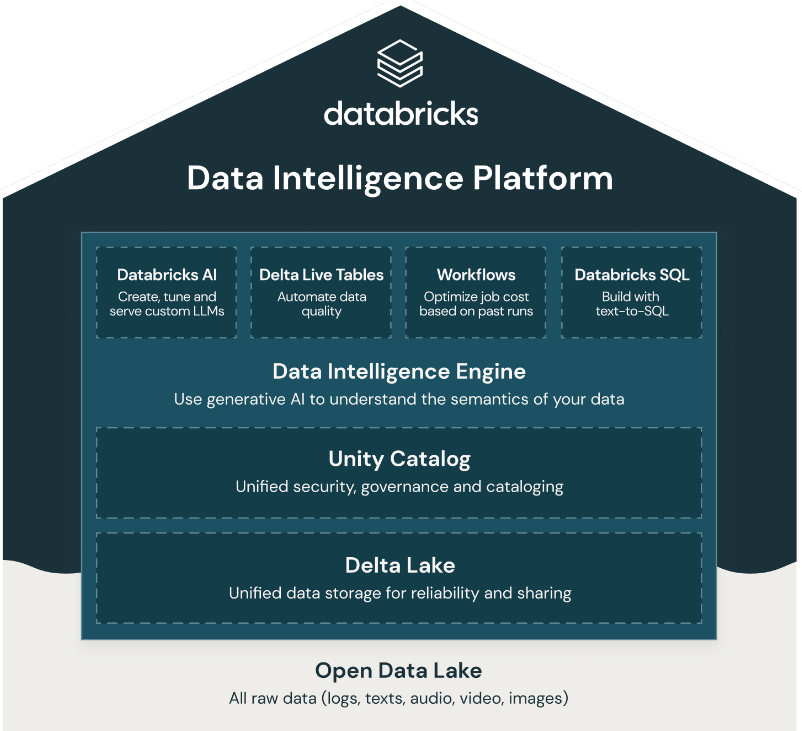
\includegraphics[width=\textwidth,height=.75\textheight,keepaspectratio]{./Figures/chapter-04/databricks_data_intelligence.png}};
		  % Place text and arrow
		  \draw[<-, thick] (image) -- ++(4,1) node[right, align=left,font=\small, text=gray] {Photo copied from\\ \url{https://www.datanami.com}};
		\end{tikzpicture}
		\captionof{figure}{Databricks Analytics Platform}
	\end{minipage}
\end{frame}

\begin{frame}
\centering % Center the content horizontally
\vfill % Center the content vertically
\Large{Do You Need Databricks to Work with Spark?} % Large font size for the question
\vfill % Add space at the bottom to keep the text centered vertically
\end{frame}

\begin{frame}
\centering % Center the content horizontally
\vfill % Center the content vertically
\Large{Do You Need Databricks to Work with Spark?} % Question in normal color
\vspace{1em} % Add some vertical space before the answer
%\Large{\textcolor{red}{\textbf{NO}}} % Answer "NO" in red and bold for emphasis
\vfill % Add space at the bottom to keep the text centered vertically
\end{frame}

\begin{frame}
\centering % Center the content horizontally
\vfill % Center the content vertically
\Large{Do You Need Databricks to Work with Spark?} % Question in normal color
\hspace{1cm} % Add some vertical space before the answer
\Large{\textcolor{blue}{The answer is NO!}} % Answer "NO" in red and bold for emphasis
\vfill % Add space at the bottom to keep the text centered vertically
\end{frame}


\begin{frame}
\frametitle{Do You Need Databricks to Work with Spark?}

\begin{itemize}
  \item Spark workloads can be run both on the Cloud and on-premise.
  \begin{itemize}
    \item \textbf{Cloud:} Choose any preferred cloud provider, like AWS, GCP, or Azure.
    \item \textbf{On-Premise:} Deploy on Kubernetes or utilize big data distributions such as Cloudera.
    \item \textbf{Serverless Platforms:} For efficient resource management, consider options like:
    \begin{itemize}
      \item \textbf{AWS:} EMR Serverless or AWS Glue for auto-scaling and managed services.
      \item \textbf{GCP:} Dataproc for integrated analytics and machine learning.
      \item \textbf{Azure:} Azure Synapse for big data and advanced analytics.
    \end{itemize}
  \end{itemize}
\end{itemize}
\end{frame}

%%%%%%%%%%%%%%%%%%%%%%%%%%%%%%%%%%%%%%%%%%%%%%%%%%%%%%
\subsection{Apache Spark in Data Platforms}

\begin{frame}{Technical components in a data lake}
	\begin{minipage}{\textwidth}
		\begin{tikzpicture}
		  % Place image at the left side
		  \node[anchor=west] (image) at (0,0) {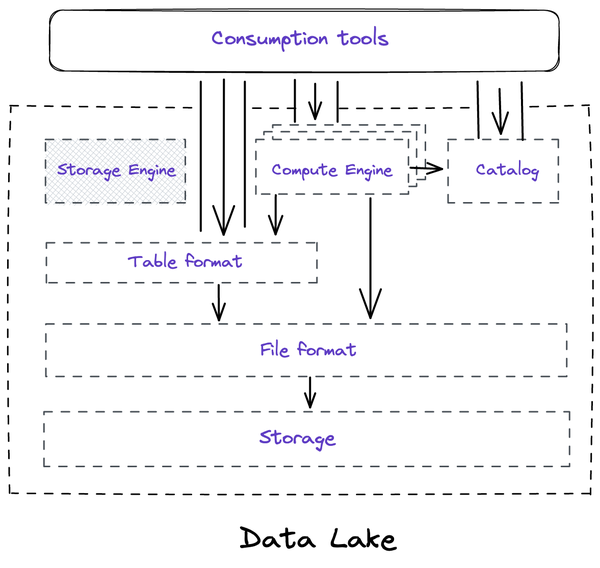
\includegraphics[width=\textwidth,height=.75\textheight,keepaspectratio]{./Figures/chapter-03/datalake_table_format.png}};
		  % Place text and arrow
		  \draw[<-, thick] (image) -- ++(4,1) node[right, align=left,font=\small, text=gray] {Apache Iceberg: The Definitive Guide: \\Data Lakehouse Functionality,\\ Performance, and Scalability\\ on the Data Lake\\ PUBLISHED BY:
		  O'Reilly Media, Inc.};
		\end{tikzpicture}
		\captionof{figure}{Technical components in a data lake}
	\end{minipage}
\end{frame}

%%%%%%%%%%%%%%%%%%%%%%%%%%%%%%%%%%%%%%%%%%%%%%%%%%%%%%
\begin{frame}{Technical components in a data lake}
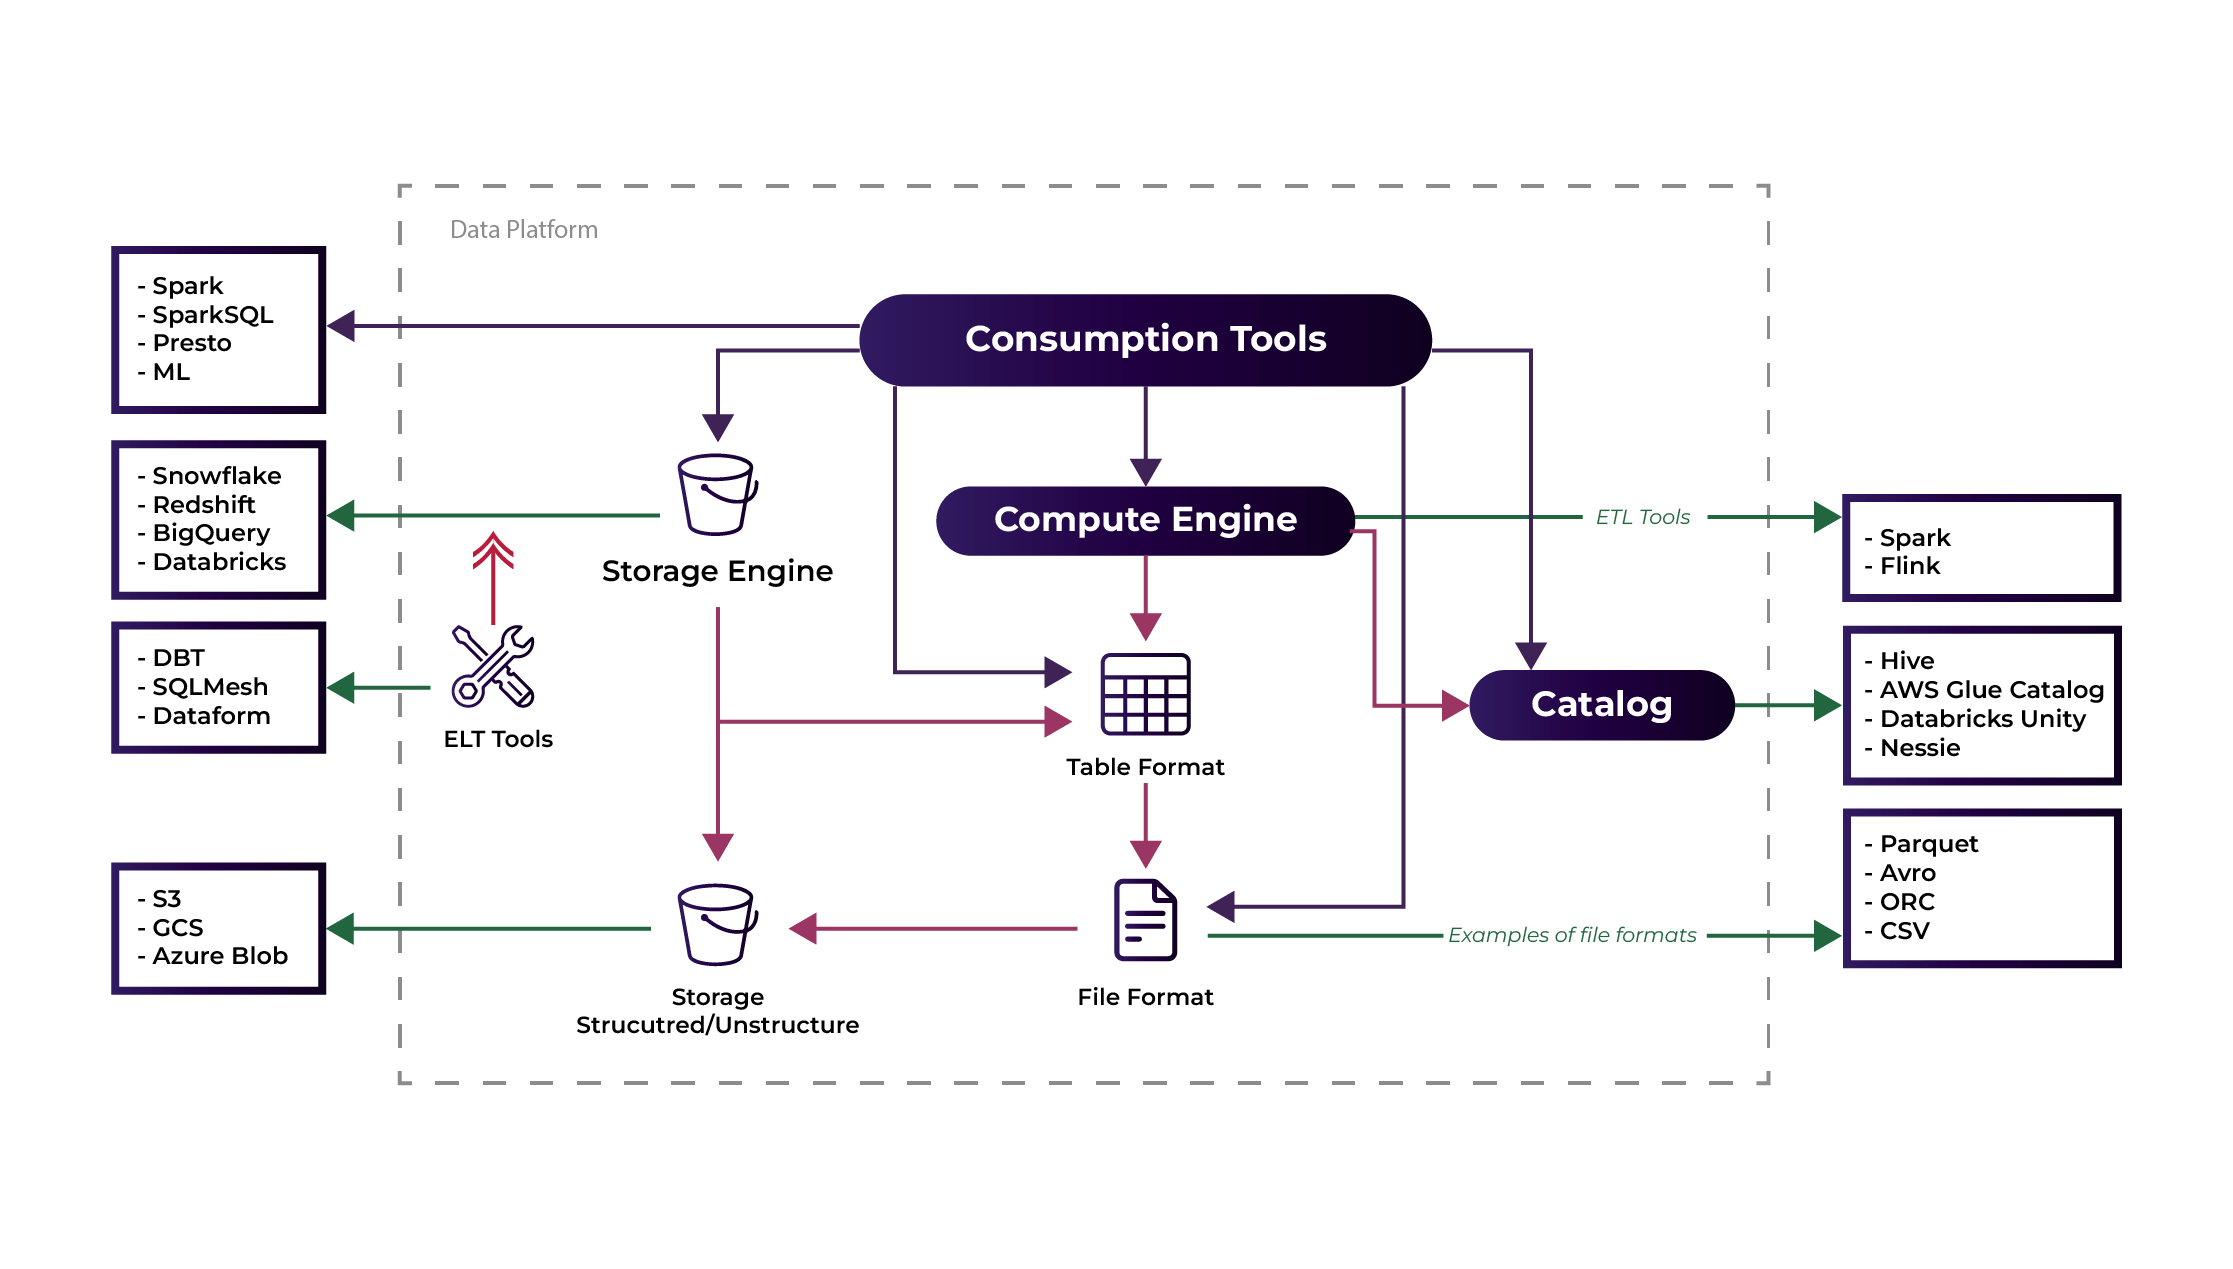
\includegraphics[width=\textwidth,height=.8\textheight,keepaspectratio]{./Figures/chapter-04/DataPlatform.png};
\end{frame}
%%%%%%%%%%%%%%%%%%%%%%%%%%%%%%%%%%%%%%%%%%%%%%%%%%%%%%
\subsection{Running Spark}
\begin{frame}
\frametitle{Running Spark for Beginners}

\begin{itemize}
  \item \textbf{Databricks Community Edition:} The simplest option for Spark beginners. A free version that's easy to use for learning and small projects. \pause
  \item \textbf{Install Spark Locally:} For hands-on experience with Spark's core features on your own machine. \pause
  \item \textbf{Spark on Docker:} For a flexible, containerized environment that can replicate a production setup.
\end{itemize}

\bigskip % Adds a bit more vertical space

\emph{Note:} For those new to Spark, starting with the Databricks Community Edition is highly recommended due to its user-friendly interface and comprehensive documentation.

\end{frame}
\begin{frame}
\centering % Center the content horizontally
\vfill % Center the content vertically
\Large{Demo!} % Large font size for the question
\vfill % Add space at the bottom to keep the text centered vertically
\end{frame}

%%%%%%%%%%%%%%%%%%%%%%%%%%%%%%%%%%%%%%%%%%%%%%%%%%%%%%
\subsection{From MapReduce to Apache Spark}

%%%%%%%%%%%%%%%%%%%%%%%%%%%%%%%%%%%%%%%%%%%%%%%%%%%%%%
\begin{frame}
	\frametitle{The basic idea of MapReduce}
	\begin{itemize}  [<+->]
		\item Assume we need to launch a high-throughput bulk-production sandwich shop.
		\item This sandwich has a lot of raw ingredients, and our target is to produce the sandwich as quickly as possible.
		\item To make the production very quickly we need to distribute the tasks between the  \textcolor{orange}{\textit{workers}}.
	\end{itemize}
	\footnotetext[1]{This example taken from  \href{https://reberhardt.com/cs110/summer-2018/lecture-notes/lecture-14/}{https://reberhardt.com/cs110/summer-2018/lecture-notes/lecture-14/}	}
\end{frame}
%%%%%%%%%%%%%%%%%%%%%%%%%%%%%%%%%%%%%%%%%%%%%%%%%%%%%%
\begin{frame}
	\frametitle{The basic idea of MapReduce}
	We break this into three stages
	\begin{itemize}  [<+->]
		\item Map.
		\item Shuffle/Group (Mapper Intermediates).
		\item Reduce
	\end{itemize}
	\footnotetext[1]{This example taken from  \href{https://reberhardt.com/cs110/summer-2018/lecture-notes/lecture-14/}{https://reberhardt.com/cs110/summer-2018/lecture-notes/lecture-14/}	}
\end{frame}
%%%%%%%%%%%%%%%%%%%%%%%%%%%%%%%%%%%%%%%%%%%%%%%%%%%%%%
\begin{frame}
	\frametitle{Map}
	We distribute our raw ingredients amongst the workers.
	\begin{figure}
		\includegraphics[width=.5\textwidth,height=.6\textheight]{./Figures/chapter-02/map-reduce-map-side.jpeg}
	\end{figure}
	\footnotetext[1]{{\tiny This example taken from  \href{https://reberhardt.com/cs110/summer-2018/lecture-notes/lecture-14/}{https://reberhardt.com/cs110/summer-2018/lecture-notes/lecture-14/}	} }
\end{frame}
%%%%%%%%%%%%%%%%%%%%%%%%%%%%%%%%%%%%%%%%%%%%%%%%%%%%%%
\begin{frame}
	\frametitle{Shuffle/Group}
	We will organise and group the processed ingredients into piles, so that making a sandwich becomes easy.
		\begin{figure}
		\includegraphics[width=.7\textwidth,height=.6\textheight]{./Figures/chapter-02/map-reduce-shuffle.png}
	\end{figure}
	\footnotetext[1]{{\tiny This example taken from  \href{https://reberhardt.com/cs110/summer-2018/lecture-notes/lecture-14/}{https://reberhardt.com/cs110/summer-2018/lecture-notes/lecture-14/}	}}
\end{frame}
%%%%%%%%%%%%%%%%%%%%%%%%%%%%%%%%%%%%%%%%%%%%%%%%%%%%%%
\begin{frame}
	\frametitle{Reduce}
	we’ll combine the ingredients into a sandwich
	\begin{figure}
		\includegraphics[width=.96\textwidth,height=.6\textheight]{./Figures/chapter-02/map-reduce-reduce-side.png}
	\end{figure}
	\footnotetext[1]{ {\tiny This example taken from  \href{https://reberhardt.com/cs110/summer-2018/lecture-notes/lecture-14/}{https://reberhardt.com/cs110/summer-2018/lecture-notes/lecture-14/}	}}
\end{frame}
%%%%%%%%%%%%%%%%%%%%%%%%%%%%%%%%%%%%%%%%%%%%%%%%%%%%%%
\begin{frame}
	\frametitle{Map Reduce Bottelneck}
	\begin{figure}
		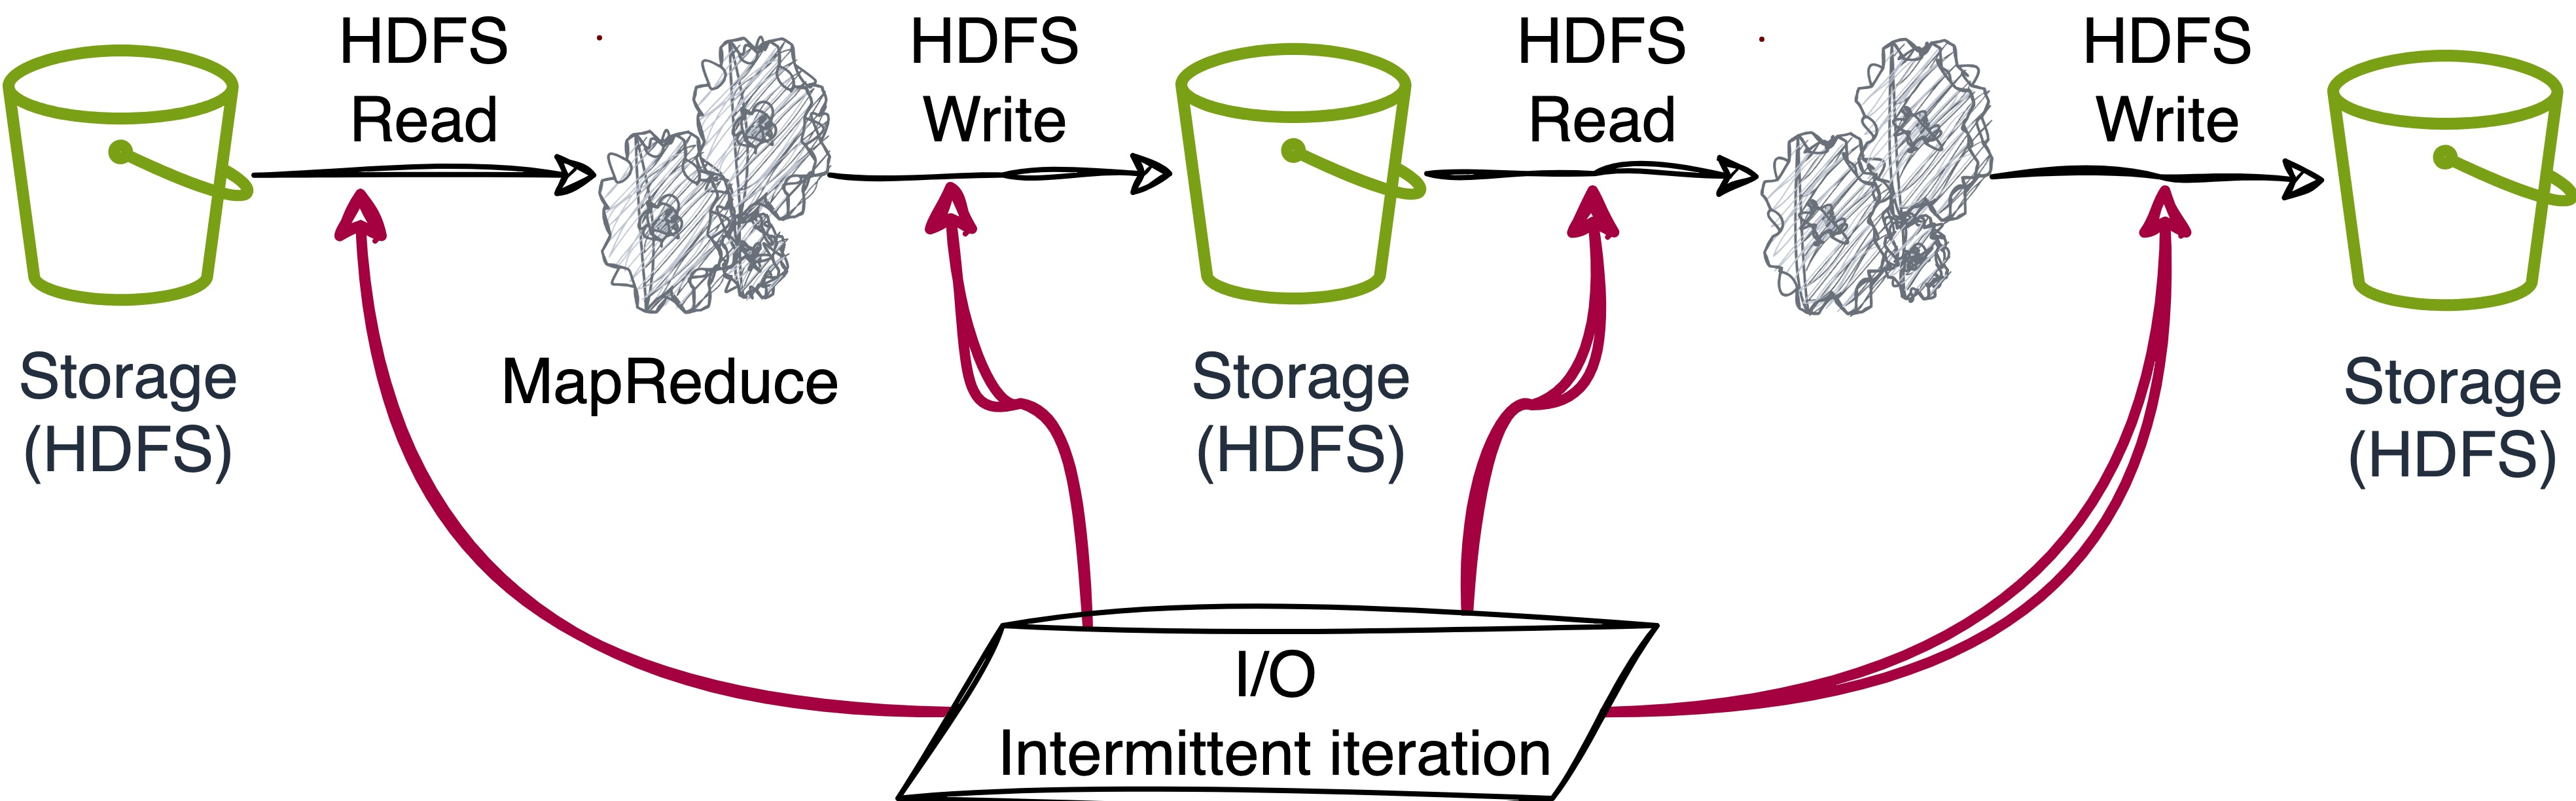
\includegraphics[width=.96\textwidth,height=.6\textheight]{./Figures/chapter-04/MR}
	\end{figure}
\end{frame}
%%%%%%%%%%%%%%%%%%%%%%%%%%%%%%%%%%%%%%%%%%%%%%%%%%%%%%
\begin{frame}
	\frametitle{Spark Motivation}
	\begin{itemize}

\item In-Memory Processing.

\item Resilient Distributed Datasets (RDDs).%**: Spark uses RDDs to perform parallel operations on data stored across cluster nodes, minimizing disk I/O by keeping data in RAM.

\item Optimized Execution.%: The DAG execution engine organizes computations efficiently, reducing unnecessary operations and combining tasks to lower data movement.

\item Caching.%: Spark allows for the caching of intermediate data in memory, benefiting iterative algorithms that reuse data, thereby avoiding repetitive disk access.

\item Advanced Optimization.%: With components like the Catalyst optimizer and Tungsten for memory and CPU efficiency, Spark streamlines execution, making it ideal for fast, iterative processing over big data.

	\end{itemize}
\end{frame}
%%%%%%%%%%%%%%%%%%%%%%%%%%%%%%%%%%%%%%%%%%%%%%%%%%%%%%
\subsection{What is Apache Spark}
\begin{frame}
\frametitle{\subsecname}
\begin{itemize}
	\item Speed. \pause
	\item Ease of use. \pause
	\item Modularity. \pause
	\item Extensibility. \pause
\end{itemize}
\end{frame}
%%%%%%%%%%%%%%%%%%%%%%%%%%%%%%%%%%%%%%%%%%%%%%%%%%%%%%
\section{Apache Spark Distributed Execution}
\begin{frame}
\frametitle{Apache Spark Distributed Execution}
\begin{itemize}
	\item Spark driver. \pause
	\item Spark session. \pause
	\item Cluster manager. \pause
	\item Spark executors. \pause
	\item Deployment mode. \pause
	\item Data partition. \pause
\end{itemize}
\end{frame}
%%%%%%%%%%%%%%%%%%%%%%%%%%%%%%%%%%%%%%%%%%%%%%%%%%%%%%
\subsection{Further Readings and Assignment}

%%% Local Variables:
%%% mode: latex
%%% TeX-master: "../main"
% !TeX root = ../main.tex
%%% TeX-engine: xetex
%%% End: